% Options for packages loaded elsewhere
\PassOptionsToPackage{unicode}{hyperref}
\PassOptionsToPackage{hyphens}{url}
\documentclass[
]{article}
\usepackage{xcolor}
\usepackage{amsmath,amssymb}
\setcounter{secnumdepth}{-\maxdimen} % remove section numbering
\usepackage{iftex}
\ifPDFTeX
  \usepackage[T1]{fontenc}
  \usepackage[utf8]{inputenc}
  \usepackage{textcomp} % provide euro and other symbols
\else % if luatex or xetex
  \usepackage{unicode-math} % this also loads fontspec
  \defaultfontfeatures{Scale=MatchLowercase}
  \defaultfontfeatures[\rmfamily]{Ligatures=TeX,Scale=1}
\fi
\usepackage{lmodern}
\ifPDFTeX\else
  % xetex/luatex font selection
\fi
% Use upquote if available, for straight quotes in verbatim environments
\IfFileExists{upquote.sty}{\usepackage{upquote}}{}
\IfFileExists{microtype.sty}{% use microtype if available
  \usepackage[]{microtype}
  \UseMicrotypeSet[protrusion]{basicmath} % disable protrusion for tt fonts
}{}
\makeatletter
\@ifundefined{KOMAClassName}{% if non-KOMA class
  \IfFileExists{parskip.sty}{%
    \usepackage{parskip}
  }{% else
    \setlength{\parindent}{0pt}
    \setlength{\parskip}{6pt plus 2pt minus 1pt}}
}{% if KOMA class
  \KOMAoptions{parskip=half}}
\makeatother
\usepackage{longtable,booktabs,array}
\usepackage{calc} % for calculating minipage widths
% Correct order of tables after \paragraph or \subparagraph
\usepackage{etoolbox}
\makeatletter
\patchcmd\longtable{\par}{\if@noskipsec\mbox{}\fi\par}{}{}
\makeatother
% Allow footnotes in longtable head/foot
\IfFileExists{footnotehyper.sty}{\usepackage{footnotehyper}}{\usepackage{footnote}}
\makesavenoteenv{longtable}
\usepackage{graphicx}
\makeatletter
\newsavebox\pandoc@box
\newcommand*\pandocbounded[1]{% scales image to fit in text height/width
  \sbox\pandoc@box{#1}%
  \Gscale@div\@tempa{\textheight}{\dimexpr\ht\pandoc@box+\dp\pandoc@box\relax}%
  \Gscale@div\@tempb{\linewidth}{\wd\pandoc@box}%
  \ifdim\@tempb\p@<\@tempa\p@\let\@tempa\@tempb\fi% select the smaller of both
  \ifdim\@tempa\p@<\p@\scalebox{\@tempa}{\usebox\pandoc@box}%
  \else\usebox{\pandoc@box}%
  \fi%
}
% Set default figure placement to htbp
\def\fps@figure{htbp}
\makeatother
\setlength{\emergencystretch}{3em} % prevent overfull lines
\providecommand{\tightlist}{%
  \setlength{\itemsep}{0pt}\setlength{\parskip}{0pt}}
\usepackage[]{natbib}
\bibliographystyle{plainnat}
\usepackage{bookmark}
\IfFileExists{xurl.sty}{\usepackage{xurl}}{} % add URL line breaks if available
\urlstyle{same}
\hypersetup{
  pdftitle={HealthEnv: Compiling Static Health QA Benchmarks into Executable Computer-Use Environments},
  hidelinks,
  pdfcreator={LaTeX via pandoc}}

\title{HealthEnv: Compiling Static Health QA Benchmarks into Executable
Computer-Use Environments}
\author{}
\date{}

\begin{document}
\maketitle

\section{HealthEnv: Compiling Longitudinal Health QA into Verifiable
Computer-Use
Environments}\label{healthenv-compiling-longitudinal-health-qa-into-verifiable-computer-use-environments}

\textbf{Technical report · Draft v0.1 · 11 October 2026}

HealthEnv Contributors

\subsection{Abstract}\label{abstract}

Health question-answering benchmarks compress a domain problem into a
prompt and a textual answer. Computer-use agents, by contrast, must
recover evidence from an interface, maintain state across actions,
produce an artifact, and satisfy workflow constraints. We introduce
\textbf{HealthEnv}, a compiler and runtime that expands longitudinal
health QA seeds into browser-based, stateful, and automatically
verifiable computer-use tasks. A seed is compiled into (i) a synthetic
longitudinal record state, (ii) an operational instruction, (iii) a
constrained GUI action surface, and (iv) a hidden state-based verifier.
The key design choice is a trust boundary: language models may plan or
rewrite task instructions, but gold answers and reward predicates remain
executable and deterministic.

Two properties are then measured rather than asserted. First,
\textbf{scalability with per-instance proof}: 1,200 environments are
generated deterministically, each individually shown to be solvable by
an oracle and gated by four negative controls, across three interface
surfaces assigned 400/400/400 and orthogonal to the reasoning skill.
Second, \textbf{robustness to who is driving}: because a computer-use
agent is a model \emph{plus} a loop, we evaluate the same tasks through
three independently released harnesses --- \texttt{pi}, OpenAI Codex
CLI, and DeepSeek's \texttt{dsh} --- holding the model, the task sample,
the prompt bytes, and the tool surface identical, and scoring offline so
no harness can observe correctness mid-episode. Making three CLIs run
one task non-interactively proved to be where the measurement lives: a
JSON tool-call body is silently corrupted by PowerShell, a multi-line
argv prompt is truncated to its first line, a transcript marker can be
matched against the prompt echo and kill a run on startup, and a harness
sandbox can fail closed so that a low score reflects a blocked agent
rather than a failed task. Each hazard is documented with the
measurement that exposed it.

A dependency-free reference implementation includes a
LifeAgentBench-format adapter, an OpenAI-compatible planner integration,
a sealed agent channel that cannot reach the verifier, and a
three-surface browser workbench. All 55 unit and regression tests pass;
the 1,200-environment scale run holds 1,200/1,200 oracle passes,
1,200/1,200 rejections for each of four negative controls, and zero
structural errors, with the whole corpus reachable through a real
headless browser. These experiments establish implementation correctness
and cross-harness comparability, not clinical validity or training
benefit. We conclude with the experiments required to test whether
QA-driven environment synthesis improves computer-use agents while
preserving reward fidelity and medical safety.

\subsection{1. Introduction}\label{introduction}

Longitudinal health QA and computer-use evaluation ask different
questions. A QA benchmark asks whether a model can derive an answer from
a record. A computer-use benchmark asks whether an agent can navigate a
system, locate the right evidence, update the right state, produce the
right artifact, and avoid unsafe side effects. The underlying domain
relation may be shared, but the observable behavior and failure modes
are not.

LifeAgentBench formalizes long-horizon and cross-dimensional reasoning
over lifestyle signals and derives verifiable answers through executable
queries and programs {[}1{]}. HealthAdminBench and MedCUA-Bench show
that medical computer use adds another layer: cross-system coordination,
document handling, interface grounding, workflow state, and safety
constraints {[}2, 3{]}. Meanwhile, environment-synthesis systems such as
InfiniteWeb, AutoWebWorld, GUI-GENESIS, CUA-Gym, and Gym-Anything
suggest that environments---not only trajectories---are becoming a
primary scaling axis {[}4--8{]}.

This motivates a compiler view:

\begin{quote}
A static QA item is a compressed specification of a world relation.
Expanding it into an executable environment should make the relation
observable through actions and verifiable through state.
\end{quote}

HealthEnv is a first vertical slice of this idea. It accepts a question,
answer, evidence relation, and record set; emits a task specification;
serves a browser interface; and scores the resulting terminal state. The
present release is intentionally narrow. It demonstrates longitudinal
record review and care-note workflows, not a complete EHR, payer portal,
or clinical decision-support system.

\subsubsection{Contributions}\label{contributions}

\begin{enumerate}
\def\labelenumi{\arabic{enumi}.}
\tightlist
\item
  \textbf{QA-to-CUA compilation.} We define a concrete mapping from
  health QA seeds to stateful browser tasks with explicit actions and
  terminal conditions.
\item
  \textbf{Gold/planner separation.} Optional LLM planning can alter
  instruction wording but cannot create or modify the answer, evidence
  set, or verifier.
\item
  \textbf{A verifiable task IR.} The released schema separates public
  observations, mutable workflow state, hidden reward predicates, and
  generation provenance.
\item
  \textbf{Surfaces as a controlled variable.} Tasks compile onto three
  presentation surfaces that never change the evidence, the gold answer,
  or the verifier, so an interface-grounding failure can be
  distinguished from a reasoning failure.
\item
  \textbf{A per-instance proof at scale.} The corpus is not merely
  large; every one of the 1,200 environments is individually proved
  solvable and individually gated by four negative controls.
\item
  \textbf{Cross-harness comparability, measured.} Three independently
  released agent harnesses run the same tasks under one model, one
  sample, one prompt, and one tool surface, with five interface hazards
  documented that would otherwise have skewed the result while still
  producing plausible numbers.
\item
  \textbf{An executable reference system.} The repository includes a
  dependency-free Python runtime, a three-surface longitudinal-health
  GUI, a sealed agent channel, a LifeAgentBench-format adapter, and
  deterministic tests.
\item
  \textbf{An honest experimental boundary.} We report compiler and
  verifier validity checks and cross-harness comparability while leaving
  agent-training gains, real-software transfer, and clinical validity as
  open empirical questions.
\end{enumerate}

\subsection{2. Problem formulation}\label{problem-formulation}

Let a QA seed be

{[} x = (q, y, D, E, m), {]}

where (q) is a question, (y) is the answer, (D) is a set of longitudinal
records, (E \subseteq D) is the evidence set, and (m) is task metadata.
A compiler maps the seed to an interactive environment

{[} C(x) \rightarrow \mathcal{M} = (S, A, T, O, R), {]}

where (S) is workflow state, (A) is the action space, (T) is a
deterministic transition function, (O) is the browser observation, and
(R) is a state-based verifier.

The compilation is useful only if it satisfies four properties:

\begin{itemize}
\tightlist
\item
  \textbf{Semantic preservation:} success in the environment entails
  recovering the relation encoded by the QA item.
\item
  \textbf{Action necessity:} the answer cannot be obtained by copying a
  visible gold label; the agent must interact with evidence and workflow
  state.
\item
  \textbf{Verifier fidelity:} reward depends on the intended state, not
  on surface text alone.
\item
  \textbf{Isolation:} generated tasks contain no real patient data and
  do not expose hidden gold state to the agent.
\end{itemize}

\subsection{3. System design}\label{system-design}

\begin{figure}
\centering
\pandocbounded{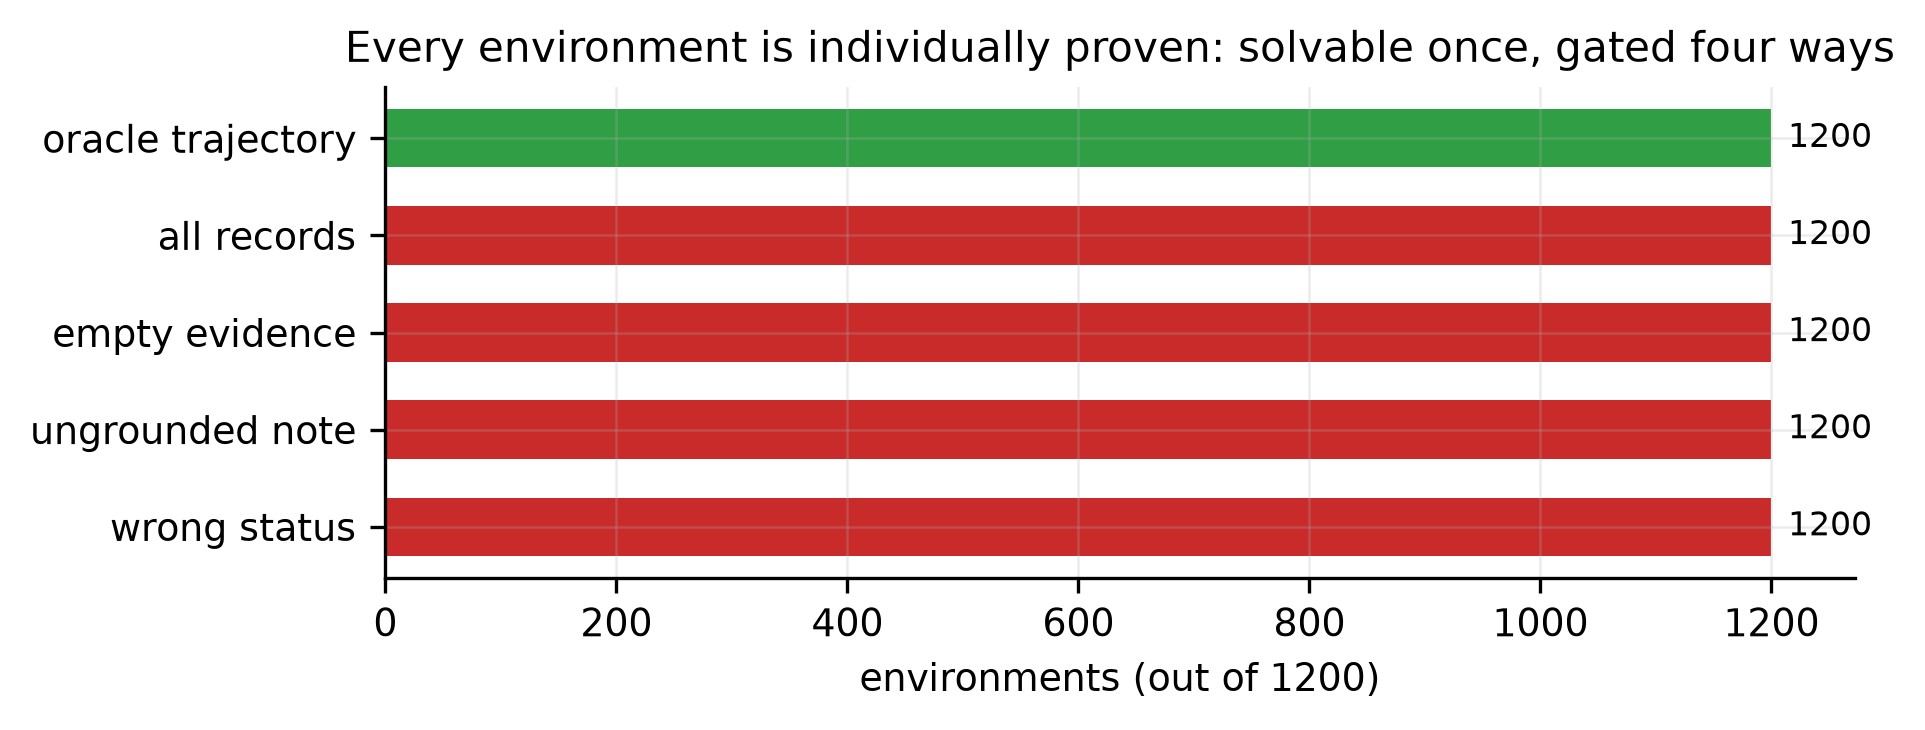
\includegraphics[keepaspectratio,alt={The compilation pipeline. A QA seed fixes domain truth; an optional planner may reword the instruction but never touches the answer or verifier; the compiled task is served as a browser surface and scored by a deterministic state verifier.}]{figures/fig1-pipeline.png}}
\caption{The compilation pipeline. A QA seed fixes domain truth; an
optional planner may reword the instruction but never touches the answer
or verifier; the compiled task is served as a browser surface and scored
by a deterministic state verifier.}
\end{figure}

\subsubsection{3.1 Seed schema}\label{seed-schema}

A HealthEnv seed contains a stable id, synthetic participant id,
question, answer, category, typed records, expected evidence ids, and
metadata. The current compiler supports numeric comparisons, temporal
aggregation, and cross-dimensional selection. Records are deliberately
simple JSON objects so adapters can be written without importing a
healthcare data model.

The public demo uses only synthetic records. The LifeAgentBench adapter
reads a local upstream checkout and synthesizes a new record state that
preserves the QA relation. This choice avoids redistributing upstream
payloads from a repository for which a license was not detected during
development.

\subsubsection{3.2 Compiler}\label{compiler}

The deterministic compiler performs five steps:

\begin{enumerate}
\def\labelenumi{\arabic{enumi}.}
\tightlist
\item
  validate identifiers, record uniqueness, evidence membership, and
  status values;
\item
  construct a stable task id from the benchmark and seed id;
\item
  create a workflow instruction that requires evidence selection, note
  writing, status assignment, and submission;
\item
  derive verifier terms from explicitly configured metadata or the
  answer type;
\item
  serialize source provenance and generation mode.
\end{enumerate}

The optional planner receives only the participant id, question,
category, record types, and record count. It never receives the answer
or evidence ids. Its output must contain the selection, note, and
submission operations; it is rejected if it includes the gold answer.
Any API or validation failure falls back to the deterministic
instruction.

\subsubsection{3.3 Browser environment}\label{browser-environment}

The environment exposes a two-panel workbench. The left panel contains
searchable, filterable longitudinal records. The right panel contains
evidence count, care-note editor, workflow priority, and submission
control. Source records are read-only. After submission, the runtime
rejects all mutations until reset. Accepted actions append an audit
event.

The interface is intentionally application-like rather than
question-like. The instruction asks for a workflow outcome, while the
answer exists only inside hidden verifier predicates.

\subsubsection{3.4 Verifier}\label{verifier}

The terminal verifier contains five checks:

\begin{longtable}[]{@{}lrl@{}}
\toprule\noalign{}
Check & Weight & Current predicate \\
\midrule\noalign{}
\endhead
\bottomrule\noalign{}
\endlastfoot
Evidence selection & 0.30 & Exact equality with required record ids \\
Grounded note & 0.30 & All normalized gold terms occur in the note \\
Workflow status & 0.15 & Status equals the required value \\
Submission & 0.15 & Explicit submit action occurred \\
Safety & 0.10 & No forbidden source-state edit was recorded \\
\end{longtable}

The weighted score provides process-level signal. Strict success
requires every check. Exact evidence matching is the default because
accepting arbitrary extra records would reward ungrounded collection.
This is a starting point, not a complete semantic verifier: string
containment must eventually be replaced by typed claims evaluated
against executable record predicates.

\begin{figure}
\centering
\pandocbounded{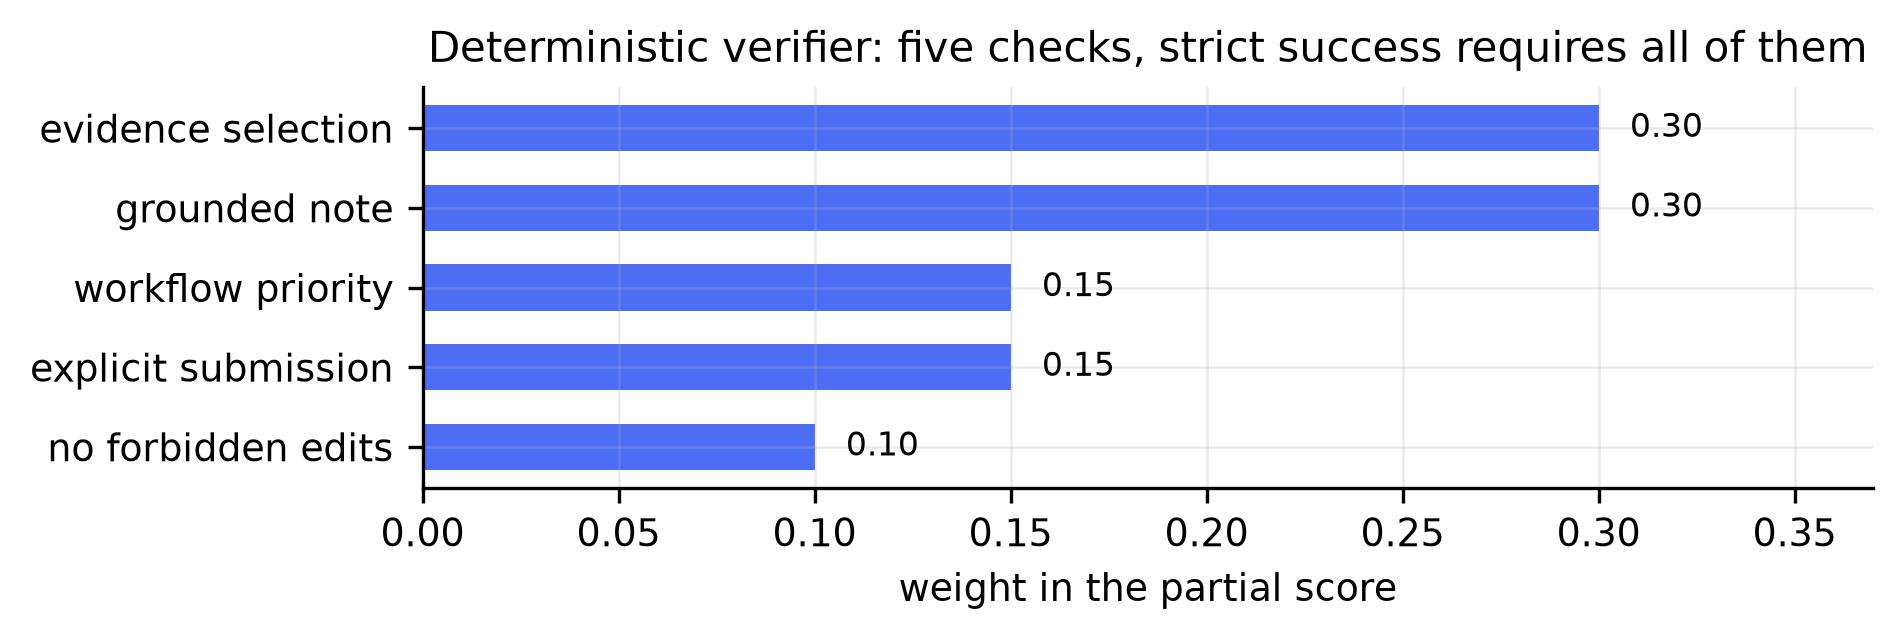
\includegraphics[keepaspectratio,alt={Verifier weights, and the role each check plays in separating a reasoning failure (0.70) from a harness that cannot run (0.10).}]{figures/fig5-verifier.png}}
\caption{Verifier weights, and the role each check plays in separating a
reasoning failure (0.70) from a harness that cannot run (0.10).}
\end{figure}

\subsubsection{3.5 Trust boundaries}\label{trust-boundaries}

HealthEnv separates three roles that environment-synthesis pipelines
often blur:

\begin{itemize}
\tightlist
\item
  the \textbf{seed} defines domain truth;
\item
  the \textbf{planner} defines how the task is communicated;
\item
  the \textbf{verifier} defines success over state.
\end{itemize}

The planner cannot modify the verifier. The browser cannot read the
verifier. The agent cannot mutate source records. The compiler logs
whether an LLM was used and whether gold state remained deterministic.

\subsubsection{3.6 Interface surfaces}\label{interface-surfaces}

A benchmark that renders every task through one layout measures that
layout. We therefore compile each seed onto one of three surfaces:

\begin{longtable}[]{@{}
  >{\raggedright\arraybackslash}p{(\linewidth - 4\tabcolsep) * \real{0.3333}}
  >{\raggedright\arraybackslash}p{(\linewidth - 4\tabcolsep) * \real{0.3333}}
  >{\raggedright\arraybackslash}p{(\linewidth - 4\tabcolsep) * \real{0.3333}}@{}}
\toprule\noalign{}
\begin{minipage}[b]{\linewidth}\raggedright
Surface
\end{minipage} & \begin{minipage}[b]{\linewidth}\raggedright
Presentation
\end{minipage} & \begin{minipage}[b]{\linewidth}\raggedright
Observation shape
\end{minipage} \\
\midrule\noalign{}
\endhead
\bottomrule\noalign{}
\endlastfoot
\texttt{timeline} & reverse-chronological row list & one row per
record \\
\texttt{vitals-dashboard} & signal tiles with large readings & one card
per record \\
\texttt{clinical-ledger} & dense table with checkboxes & one table row
per record \\
\end{longtable}

The surface is assigned deterministically at seed time and travels with
the task. It is a property of \textbf{presentation only}: a surface
never changes the record set, the gold evidence, the required note
terms, or the verifier weights. The three surfaces are assigned
400/400/400 across the corpus and are orthogonal to the reasoning skill,
so a difference between surfaces cannot be explained by task difficulty.

This separation matters because it makes one specific confound
measurable. If a harness degrades on \texttt{clinical-ledger} but not on
\texttt{timeline}, the failure is interface grounding rather than
reasoning. Two engineering defects found during development were exactly
of this kind and would have been invisible under a single layout:

\begin{itemize}
\tightlist
\item
  The runtime's public task projection whitelisted fields and silently
  dropped \texttt{surface}, so every task rendered as \texttt{timeline}
  regardless of what the compiler had assigned. The data was correct and
  only the presentation was wrong.
\item
  The ledger row template omitted the \texttt{data-record-id} attribute,
  so a click selected \texttt{undefined} and the evidence counter never
  advanced. The initial working surfaces hid a control that did not
  work.
\end{itemize}

Both are recorded here because they are the class of defect that
surface-conditioned evaluation is meant to surface, and because neither
was detectable from the compiler's own tests.

A third defect of the same class surfaced during the full-corpus browser
run, and it is the reason the browser proof is run over all 1200 tasks
rather than a sample. The first full run returned 1198/1200: two tasks
reported the evidence set correct but the submitted note empty, while
replaying the identical action sequence against the same task offline
reached strict success --- the environment and verifier were correct,
and the browser layer was not. The cause was in the front-end: two
change handlers (\texttt{set\_note}, \texttt{set\_status}) issued their
\texttt{fetch} calls without ordering, and when the responses resolved
out of order the first response's form sync restored the note textarea
from a snapshot that predates the other write, so the submitted note was
silently empty. Serializing the front-end action chain and re-running
the full corpus gave 1200/1200. A dedicated A/B probe (120 repeated
episodes per arm on the two originally failing tasks) showed the failure
only under the unserialized front-end; the fix also carries a regression
test asserting the served HTML keeps \texttt{act()} serialized. The
honest caveat is statistical: at an observed rate of 2/1200, a
120-episode probe cannot prove the race was the \emph{only} cause ---
what the three consistent measurements establish is that the serialized
front-end reaches 1200/1200 where the unserialized one does not.

\subsubsection{3.7 A sealed agent channel}\label{a-sealed-agent-channel}

An evaluated agent must not be able to read the verifier. The original
runtime exposed a single \texttt{/api/verify} endpoint that returned a
check-by-check report, and that report named the required evidence ids.
An agent that could reach it would not need to reason: it could read the
answer, satisfy the checks one at a time, and hill-climb against the
gold oracle without ever generalizing.

The released system therefore exposes two distinct channels:

\begin{itemize}
\tightlist
\item
  a \textbf{demo channel} (\texttt{/api/task}, \texttt{/api/action},
  \texttt{/api/verify}) used by the interactive workbench, where
  verification feedback is the point; and
\item
  a \textbf{sealed agent channel} (\texttt{/api/agent/task},
  \texttt{/api/agent/action}, \texttt{/api/agent/state}) that the
  evaluated harnesses actually use.
\end{itemize}

The agent channel applies an explicit projection: the response carries
the instruction, the participant header, and the records, and nothing
else. The reasoning \texttt{category} is stripped because it names the
skill under test, and the \texttt{surface} is stripped because it
correlates with it. Most importantly, \texttt{submit} on the agent
channel returns \texttt{\{"ok":\ true,\ "submitted":\ true\}} and
\textbf{no verification payload at all}. Scoring happens offline, after
the episode ends, so a harness cannot observe correctness mid-episode or
steer toward it. Regression tests assert that \texttt{/api/verify},
\texttt{/api/task}, and \texttt{/api/state} are all \texttt{404} on the
tool server an agent can reach.

\subsection{4. Prototype evaluation}\label{prototype-evaluation}

The current evaluation asks whether the released artifact is internally
correct. It does not ask whether a trained CUA generalizes better.

\subsubsection{4.1 Tasks}\label{tasks}

We construct three privacy-safe QA seeds:

\begin{enumerate}
\def\labelenumi{\arabic{enumi}.}
\tightlist
\item
  a two-day oxygen-saturation comparison;
\item
  a three-night sleep-duration aggregation;
\item
  a joint activity-and-stress selection across dates.
\end{enumerate}

Each seed includes distractors. Compilation produces one executable JSON
task per seed.

\subsubsection{4.2 Tests}\label{tests}

We evaluate:

\begin{itemize}
\tightlist
\item
  schema rejection for unknown evidence;
\item
  deterministic compilation and round-trip parsing;
\item
  gold-answer non-leakage in default instructions;
\item
  positive oracle execution;
\item
  rejection of missing evidence, extra distractors, and forbidden edits;
\item
  transactional runtime behavior after submission;
\item
  end-to-end compilation of all three seeds.
\end{itemize}

\subsubsection{4.3 Results}\label{results}

\begin{longtable}[]{@{}
  >{\raggedright\arraybackslash}p{(\linewidth - 2\tabcolsep) * \real{0.4286}}
  >{\raggedleft\arraybackslash}p{(\linewidth - 2\tabcolsep) * \real{0.5714}}@{}}
\toprule\noalign{}
\begin{minipage}[b]{\linewidth}\raggedright
Measure
\end{minipage} & \begin{minipage}[b]{\linewidth}\raggedleft
Result
\end{minipage} \\
\midrule\noalign{}
\endhead
\bottomrule\noalign{}
\endlastfoot
Unit and regression tests & 55 / 55 pass \\
Seeds compiled & 3 / 3 \\
Oracle strict success & 3 / 3 \\
Missing-evidence mutations rejected & 3 / 3 \\
Scale run: environments generated and compiled & 1200 \\
Scale run: unique task ids & 1200 \\
Scale run: oracle strict passes & 1200 / 1200 \\
Scale run: negative controls rejected & 1200 / 1200 (four controls) \\
Scale run: structural errors & 0 \\
Scale run in a real headless browser (all 1200 tasks) & 1200 / 1200
strict; 0 JS/network failures \\
LifeAgentBench-format adapter smoke & strict success 1.0 \\
TierFlow \texttt{tierflow\_pro} planner & 3 / 3; zero fallbacks; gold
unchanged \\
Real headless-browser workflow & 100\%; zero JS/network failures \\
Missing-evidence score & 0.70 \\
Runtime dependencies & 0 \\
\end{longtable}

A score of 0.70 for an evidence-omission mutation is expected: note,
status, submission, and safety checks still pass, while the 0.30
evidence check fails. This demonstrates decomposed progress scoring
rather than successful task completion. The optional TierFlow path
planned all three instructions with \texttt{tierflow\_pro} without
fallback; every artifact records \texttt{llm\_used\_for\_gold:\ false}.
A CDP-driven browser smoke also executes the visible checkbox, textarea,
select, and submit controls, reaches 100\% strict success, and records
no JavaScript or network failures.

The browser proof is run over the \textbf{entire corpus}, not a sample:
all 1200 compiled tasks are booted one chunk at a time, driven through a
real headless browser (navigate, click the toolbar controls, select
evidence, type the note, set the priority, submit), and asserted to
reach strict success with no JavaScript or network errors. The committed
run is 1200/1200 across all three surfaces and all seven reasoning
skills, and it is the run that exposed the front-end ordering defect
described in Section 3.6 --- the first pass scored 1198/1200, with the
two missing tasks traced to a silent, order-dependent loss of the note
rather than to any task or verifier fault.

\subsubsection{4.4 Synthesis at scale}\label{synthesis-at-scale}

Three hand-written seeds cannot distinguish a compiler from a template.
We therefore add a deterministic generator, \texttt{healthenv.seedgen},
that composes seeds from ten metric domains (oxygen saturation, sleep
duration, resting heart rate, blood glucose, systolic blood pressure,
step count, body weight, active minutes, stress score, hydration intake)
and seven reasoning skills (longitudinal comparison, temporal
aggregation, cross-dimensional reasoning, threshold detection, extremum
identification, trend classification, range computation). A single
integer seed fixes the entire corpus.

Two properties matter more than the count itself. First, \textbf{the
answer is derived, not attached}: each generator constructs record
values so that the stated conclusion follows from them, and the compiler
turns that conclusion into the verifier's grounded-note terms. Second,
\textbf{every environment is proved individually}. For all 1200 tasks we
check that an oracle trajectory reaches strict success and that four
negative controls are rejected: selecting no evidence, selecting every
record, submitting an ungrounded note, and choosing the wrong workflow
priority. The second control is the one that makes distractors
load-bearing rather than decorative; it passes only if at least one
non-evidence record exists, which the pipeline asserts structurally.

Diversity is measured rather than assumed. The 1200 environments contain
1164 distinct questions, 641 distinct answers, and 1193 distinct
(question, answer) pairs. Distinct answers are fewer than distinct
instances because 343 tasks ask for a date, and the date space is small
by construction.

\begin{figure}
\centering
\pandocbounded{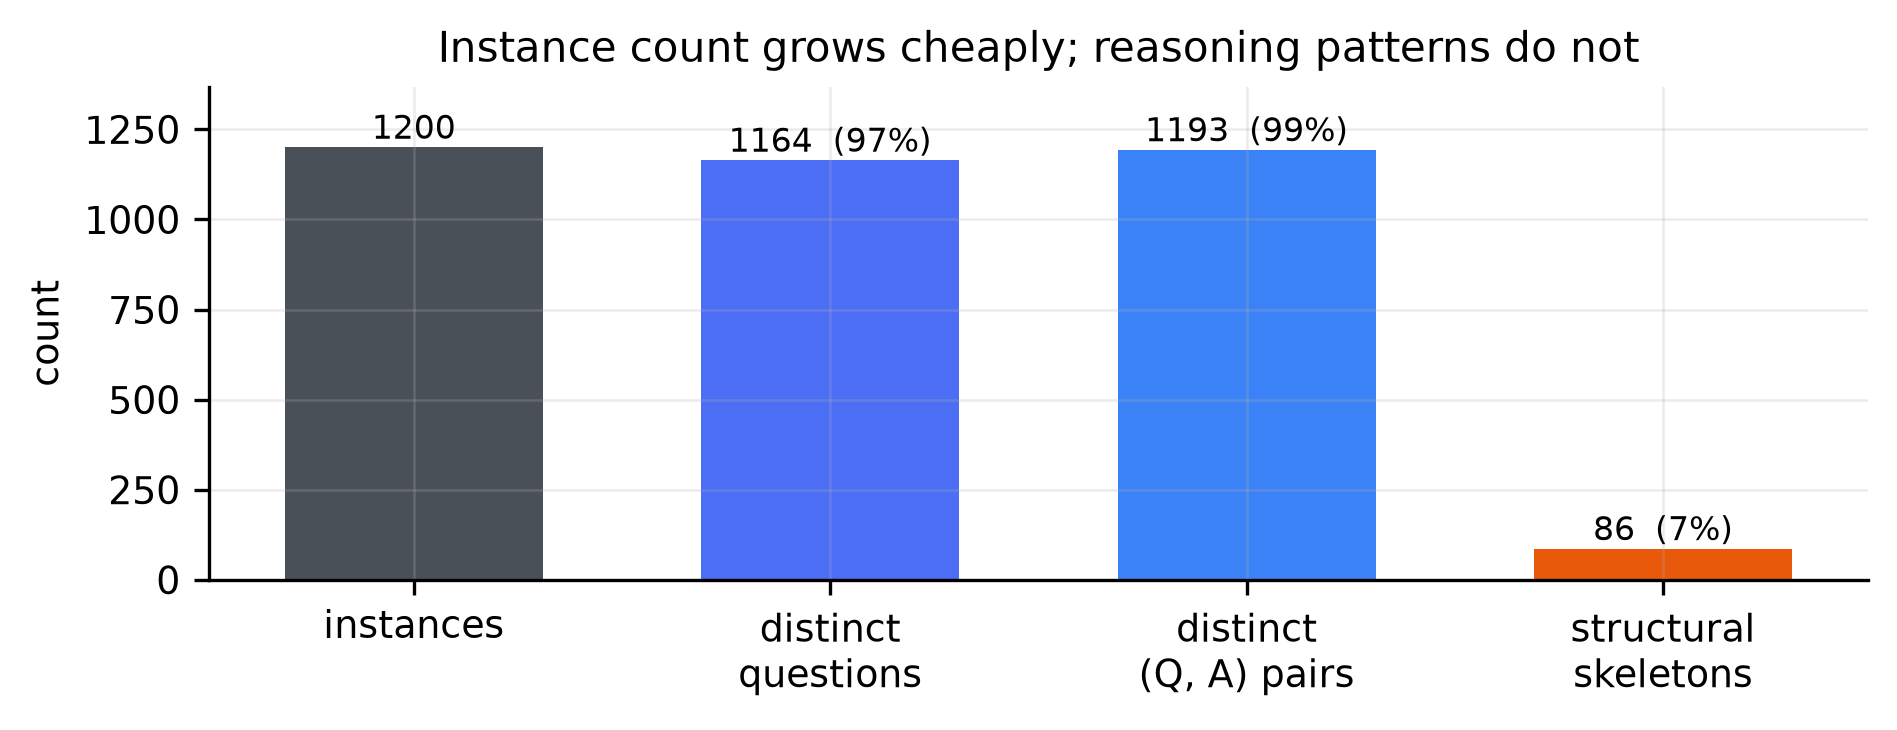
\includegraphics[keepaspectratio,alt={Instance count versus structural variety. The rightmost bar is the honest ceiling: 1200 instances occupy 86 distinct structural skeletons.}]{figures/fig2-diversity.png}}
\caption{Instance count versus structural variety. The rightmost bar is
the honest ceiling: 1200 instances occupy 86 distinct structural
skeletons.}
\end{figure}

\begin{longtable}[]{@{}lr@{}}
\toprule\noalign{}
Diversity measure & Value \\
\midrule\noalign{}
\endhead
\bottomrule\noalign{}
\endlastfoot
Distinct questions & 1164 / 1200 \\
Distinct answers & 641 / 1200 \\
Distinct (question, answer) pairs & 1193 / 1200 \\
Distinct metric combinations & 86 \\
Reasoning skills & 7 \\
Required workflow priority & review 855, routine 238, urgent 107 \\
Records per environment & 3-8 \\
Structural skeletons & 86 \\
\end{longtable}

The final row is the honest ceiling of this experiment. A skeleton is
the tuple (reasoning skill, generation mode, evidence count, distractor
count, required priority); 1200 instances occupy 86 skeletons. Raising
the instance count is a cheap operation, and reporting it alone would be
misleading: what scales easily is \emph{instances}, while what we
actually want to scale is \emph{distinct reasoning patterns and state
structures}. We therefore report both numbers together.

\subsubsection{4.5 What these results do not
show}\label{what-these-results-do-not-show}

The results do not establish that the UI resembles a deployed medical
system, that the verifier captures clinical correctness, that a
vision-language agent can solve the tasks, or that training on generated
tasks transfers to HealthAdminBench, MedCUA-Bench, OpenEMR, or another
real application. Those claims require separate experiments.

\subsection{5. Cross-harness evaluation}\label{cross-harness-evaluation}

The compiler results above establish that the environments are
well-formed. They say nothing about whether the environments
\emph{behave the same} when a different agent drives them, and that is
the question a benchmark has to answer before anyone trains on it. If a
measured difference between two agents is really a difference between
two interfaces, the benchmark is measuring the wrong thing.

\subsubsection{5.1 Why the harness is the right independent
variable}\label{why-the-harness-is-the-right-independent-variable}

A computer-use agent is not a model. It is a model plus a loop: a prompt
scaffold, a tool vocabulary, a context policy, a shell, a sandbox, and a
stop condition. Two teams can run identical weights behind different
loops and get different scores on identical tasks. Environment-synthesis
work therefore has to answer a question that QA benchmarks never face:
\textbf{is a task robust to who is driving it?}

We hold the interface fixed and vary only the driving loop. Three real,
independently released agent harnesses are evaluated:

\begin{longtable}[]{@{}
  >{\raggedright\arraybackslash}p{(\linewidth - 4\tabcolsep) * \real{0.3333}}
  >{\raggedright\arraybackslash}p{(\linewidth - 4\tabcolsep) * \real{0.3333}}
  >{\raggedright\arraybackslash}p{(\linewidth - 4\tabcolsep) * \real{0.3333}}@{}}
\toprule\noalign{}
\begin{minipage}[b]{\linewidth}\raggedright
Harness
\end{minipage} & \begin{minipage}[b]{\linewidth}\raggedright
Vendor
\end{minipage} & \begin{minipage}[b]{\linewidth}\raggedright
Loop
\end{minipage} \\
\midrule\noalign{}
\endhead
\bottomrule\noalign{}
\endlastfoot
\texttt{pi} & mariozechner/pi & coding-agent CLI with an explicit tool
allowlist \\
\texttt{codex} & OpenAI & Codex CLI, \texttt{exec} non-interactive
mode \\
\texttt{deepseek} & DeepSeek AI & \texttt{dsh} harness, headless
profile \\
\end{longtable}

\subsubsection{5.2 Controlled comparison}\label{controlled-comparison}

Four things are identical across the three harnesses, so a difference
can only be attributed to the loop:

\textbf{One model.} Every harness calls the same weights
(\texttt{tierflow\_pro}) through the same OpenAI-compatible endpoint. No
harness is advantaged by a stronger model.

\textbf{One task sample.} All three run the same 12 tasks, selected by a
stratified sampler that walks the \texttt{(surface,\ status,\ skill)}
cells rather than file order. The sample is balanced 4/4/4 across the
three surfaces and covers all seven reasoning skills.

\textbf{One prompt, byte for byte.} Every harness receives the same
instruction text, which names the tool surface and the workflow but
never the gold evidence, the note terms, or the verifier. The prompt is
written to disk and read whole by each harness (Section 5.3).

\textbf{One tool surface.} The harnesses do not get a bespoke SDK. They
call a tiny HTTP API: \texttt{get\_task}, \texttt{list\_records},
\texttt{read\_state}, \texttt{select\_record}, \texttt{set\_note},
\texttt{set\_status}, \texttt{submit}. Scoring is offline and
deterministic, computed by the same verifier after the episode ends, so
no harness can observe correctness mid-episode.

\begin{figure}
\centering
\pandocbounded{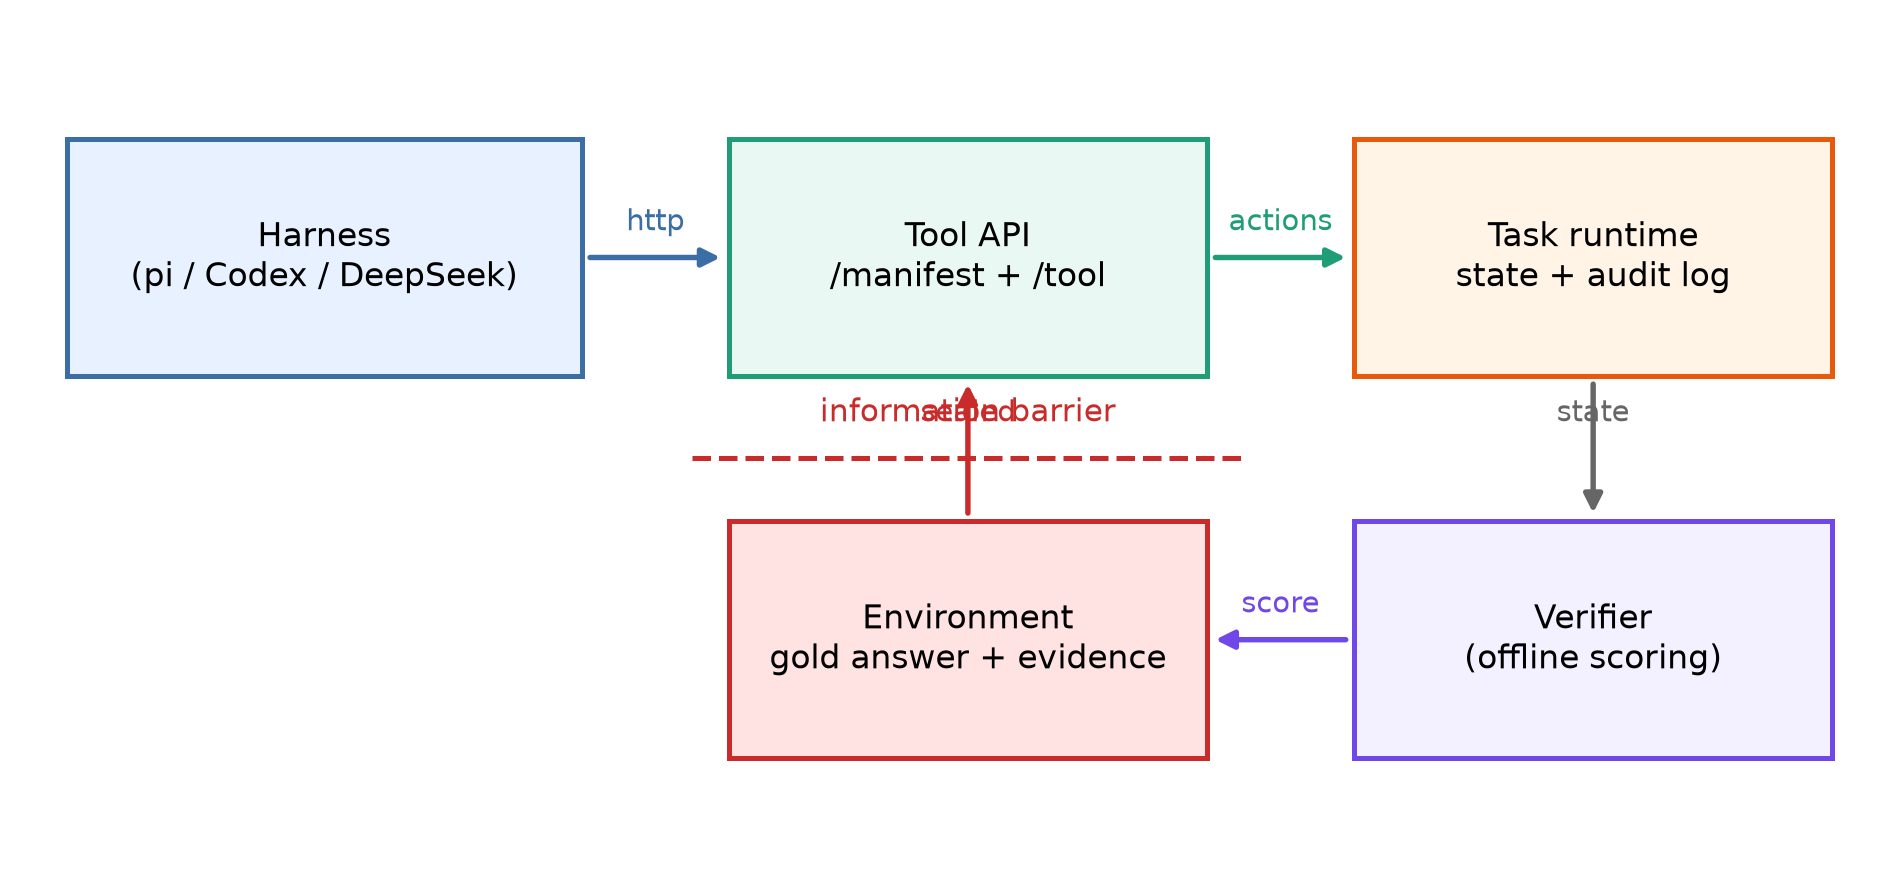
\includegraphics[keepaspectratio,alt={The controlled cross-harness workflow: one stratified task sample, one prompt, one tool surface, and offline scoring, so the only remaining variable is the driving loop.}]{figures/fig6-workflow.png}}
\caption{The controlled cross-harness workflow: one stratified task
sample, one prompt, one tool surface, and offline scoring, so the only
remaining variable is the driving loop.}
\end{figure}

\subsubsection{5.3 Interface hazards the comparison
exposed}\label{interface-hazards-the-comparison-exposed}

Getting three CLIs to run the same task non-interactively turned out to
be the empirical core of this section. Every hazard below was found by
measurement, and each one would have silently corrupted the comparison
while still producing plausible numbers.

\textbf{A JSON body is not portable across shells.} The natural way to
teach a tool call is
\texttt{curl\ -X\ POST\ \textless{}url\textgreater{}\ -d\ \textquotesingle{}\{"tool":"get\_task","args":\{\}\}\textquotesingle{}}.
Measured on this machine, that line works in bash but reaches the server
through PowerShell 5.1 as \texttt{\{tool:get\_task,args:\{\}\}} ---
PowerShell strips the inner double quotes before the native executable
sees them, so the body is no longer JSON and the call fails. This
matters because the harnesses do not share a shell: \texttt{pi} drives
Git Bash, while \texttt{codex} and \texttt{dsh} drive PowerShell. A
harness scored under this prompt would have been scored on shell
quoting. The tool surface therefore accepts a GET with query parameters,
which contains no inner quotes and is transmitted byte-identically by
both shells; the documented call is
\texttt{curl\ -s\ -G\ \textless{}url\textgreater{}/tool\ -\/-data-urlencode\ tool=\textless{}name\textgreater{}},
and POST is retained as an equivalent alias. A test asserts the two
transports return identical results.

\textbf{A multi-line argv prompt is truncated.} codex accepts the prompt
as an argv argument, and that is how it is normally invoked. On Windows
it is also silently broken: the agent received only the first line. Its
transcript shows it reasoning about an instruction it never fully got
--- ``The user says: \ldots{} This is a very vague prompt'' --- and then
spending the whole episode listing the filesystem and scanning for
listening ports instead of calling the tool API. We diagnosed this with
a sentinel prompt whose distinguishing tokens sat on lines 3 and 7 and
that asked the model to echo them back: through argv it returned
\emph{zero} of the two markers and asked for ``the follow-up lines'';
through stdin it returned both. The fix is per-harness and is recorded
on each spec: \texttt{pi} inlines the prompt with its own
\texttt{@PROMPT.txt} syntax, codex reads it from stdin, and \texttt{dsh}
--- which has no prompt-on-stdin channel --- is handed a one-line
pointer and reads the file with its own filesystem tools.

\textbf{A completion marker cannot be scraped from the transcript.}
codex and \texttt{dsh} keep a session alive after the last tool call,
which would burn the full timeout on every episode. The first fix asked
the agent to print a marker line and watched for it in the output. That
fails in a way worth recording: codex echoes the prompt to stderr, the
marker text was \emph{in} the prompt, so the watcher matched the echo
and killed the run roughly two seconds in, scoring every episode as an
empty submission. The completion signal is now read from the episode
itself --- the tool server knows the instant \texttt{submit} lands ---
with a short grace period before the process group is terminated. This
is strictly better than scraping: it is ground truth rather than a text
heuristic.

\textbf{A CLI's own shell discovery can fail where the agent lives.}
\texttt{pi} grants a \texttt{bash} tool but searches only
\texttt{C:\textbackslash{}Program\ Files\textbackslash{}Git} for the
shell; this machine's Git is installed elsewhere, so every command
failed with ``No bash shell found'' and the agent could not act at all.
A per-run project-level settings file supplies \texttt{shellPath}, so
the fix does not rewrite the user's global configuration.

\textbf{A sandbox can fail closed.} \texttt{dsh} provisions a Windows
ACL sandbox per call and, on this machine, cannot grant write access to
its own workspace (\texttt{SetNamedSecurityInfoW} fails with error 5).
Under the default \texttt{workspace-write} mode every command is refused
before it runs and the agent can only report being blocked --- a
\texttt{0.1} score that reflects the harness being unable to start, not
the harness failing the task. Its policy is set to full access, matching
what codex is given.

The general lesson is that ``the environment is deterministic'' is not
the same as ``the measurement is controlled.'' Five of these six hazards
produce a valid-looking number attached to an invalid experiment.

\subsubsection{5.4 Results}\label{results-1}

\begin{longtable}[]{@{}
  >{\raggedright\arraybackslash}p{(\linewidth - 14\tabcolsep) * \real{0.0968}}
  >{\raggedleft\arraybackslash}p{(\linewidth - 14\tabcolsep) * \real{0.1290}}
  >{\raggedleft\arraybackslash}p{(\linewidth - 14\tabcolsep) * \real{0.1290}}
  >{\raggedleft\arraybackslash}p{(\linewidth - 14\tabcolsep) * \real{0.1290}}
  >{\raggedleft\arraybackslash}p{(\linewidth - 14\tabcolsep) * \real{0.1290}}
  >{\raggedleft\arraybackslash}p{(\linewidth - 14\tabcolsep) * \real{0.1290}}
  >{\raggedleft\arraybackslash}p{(\linewidth - 14\tabcolsep) * \real{0.1290}}
  >{\raggedleft\arraybackslash}p{(\linewidth - 14\tabcolsep) * \real{0.1290}}@{}}
\toprule\noalign{}
\begin{minipage}[b]{\linewidth}\raggedright
Harness
\end{minipage} & \begin{minipage}[b]{\linewidth}\raggedleft
Episodes
\end{minipage} & \begin{minipage}[b]{\linewidth}\raggedleft
Strict success
\end{minipage} & \begin{minipage}[b]{\linewidth}\raggedleft
Mean score
\end{minipage} & \begin{minipage}[b]{\linewidth}\raggedleft
Submissions
\end{minipage} & \begin{minipage}[b]{\linewidth}\raggedleft
Timeouts
\end{minipage} & \begin{minipage}[b]{\linewidth}\raggedleft
Mean steps
\end{minipage} & \begin{minipage}[b]{\linewidth}\raggedleft
Mean elapsed
\end{minipage} \\
\midrule\noalign{}
\endhead
\bottomrule\noalign{}
\endlastfoot
pi (\texttt{pi}) & 12 & 6/12 (50\%) & 0.85 & 12 & 0 & 9.2 & 23s \\
Codex CLI (\texttt{codex}) & 12 & 7/12 (58\%) & 0.82 & 12 & 0 & 8.9 &
79s \\
DeepSeek Harness (\texttt{deepseek}) & 12 & 5/12 (42\%) & 0.78 & 12 & 0
& 9.8 & 66s \\
\end{longtable}

Across 3 harnesses and 12 episodes each, strict success ranges from 42\%
(DeepSeek Harness) to 58\% (Codex CLI) --- the same model, the same
tasks, and the same prompt bytes on every run.

On pi, strict success by rendered surface is clinical-ledger 50\%,
timeline 25\%, vitals-dashboard 75\%.

On Codex CLI, strict success by rendered surface is clinical-ledger
75\%, timeline 50\%, vitals-dashboard 50\%.

On DeepSeek Harness, strict success by rendered surface is
clinical-ledger 50\%, timeline 25\%, vitals-dashboard 50\%.

\begin{figure}
\centering
\pandocbounded{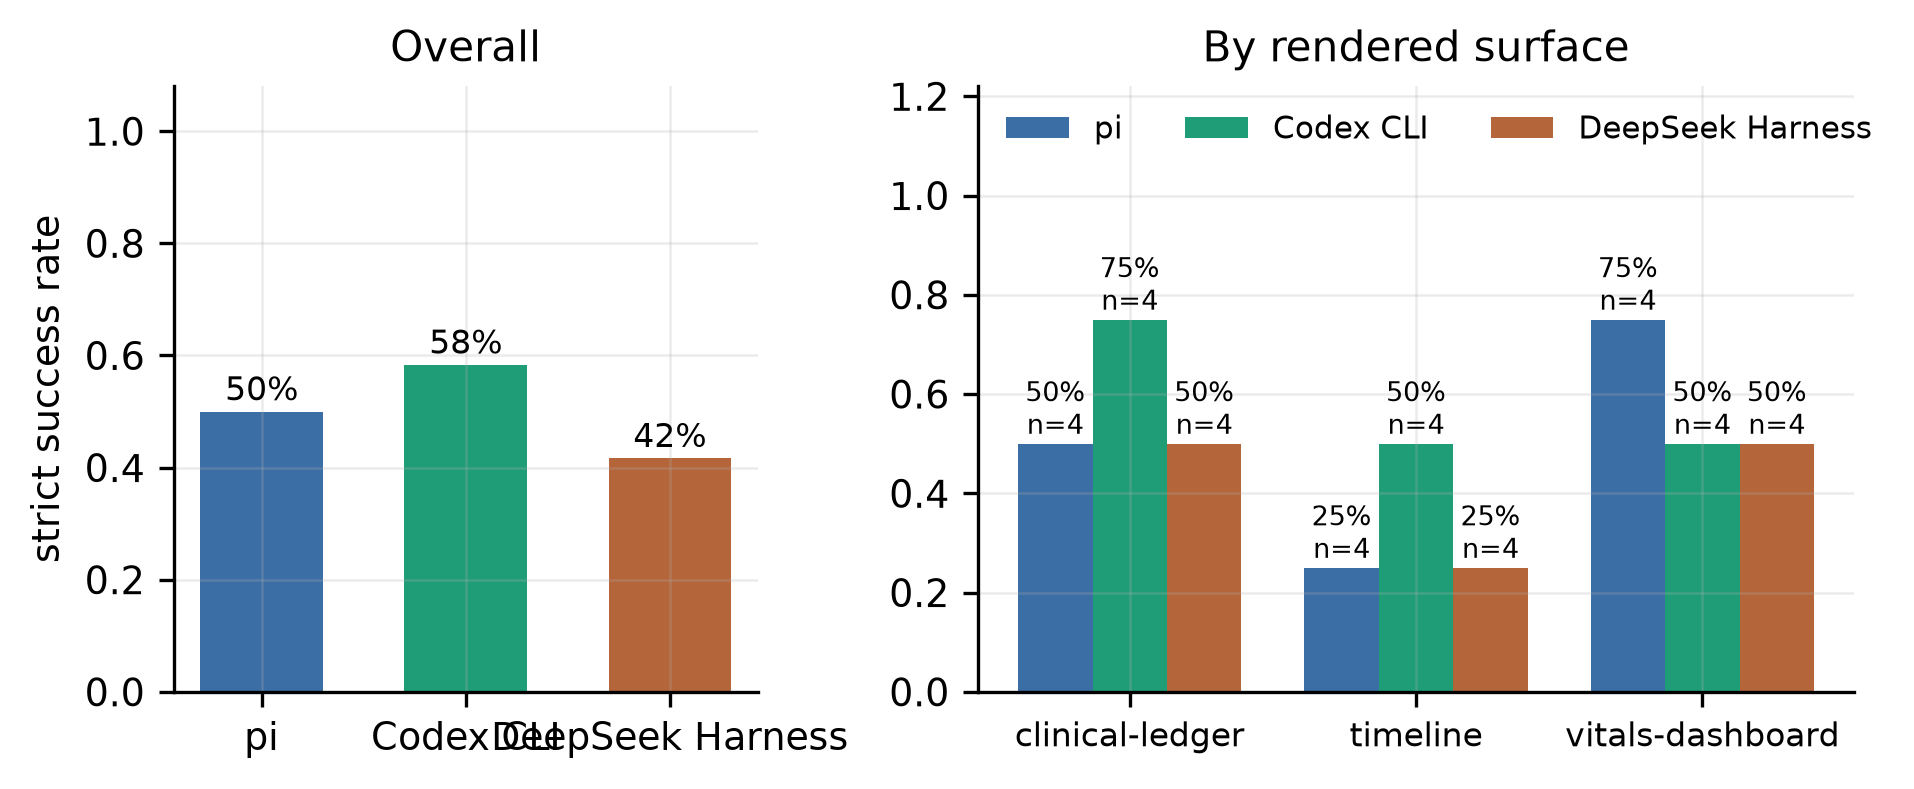
\includegraphics[keepaspectratio,alt={Strict success per harness, overall and split by rendered surface. Each surface carries an equal share of the sample, so the split tests whether a loop is sensitive to how records are presented.}]{figures/fig3-harness-success.png}}
\caption{Strict success per harness, overall and split by rendered
surface. Each surface carries an equal share of the sample, so the split
tests whether a loop is sensitive to how records are presented.}
\end{figure}

\subsubsection{5.5 Failure modes}\label{failure-modes}

\begin{longtable}[]{@{}llll@{}}
\toprule\noalign{}
Failed check & pi & Codex CLI & DeepSeek Harness \\
\midrule\noalign{}
\endhead
\bottomrule\noalign{}
\endlastfoot
evidence selection & 6/12 & 5/12 & 7/12 \\
grounded note & 0/12 & 2/12 & 2/12 \\
\end{longtable}

A score of 0.70 on a failed episode means evidence selection missed
while the note, status, submission, and safety checks still passed ---
the agent did the workflow but chose the wrong records. Episode scores
across all 36 runs were 4 at 0.40, 14 at 0.70, 18 at 1.00 --- no episode
in this run scored the 0.10 safety floor at which only the safety check
passes, so every harness could start, act, and submit. No harness solved
a range-computation task, while every harness solved
longitudinal-comparison --- the residual failures concentrate in a
reasoning skill rather than in a harness.

\begin{figure}
\centering
\pandocbounded{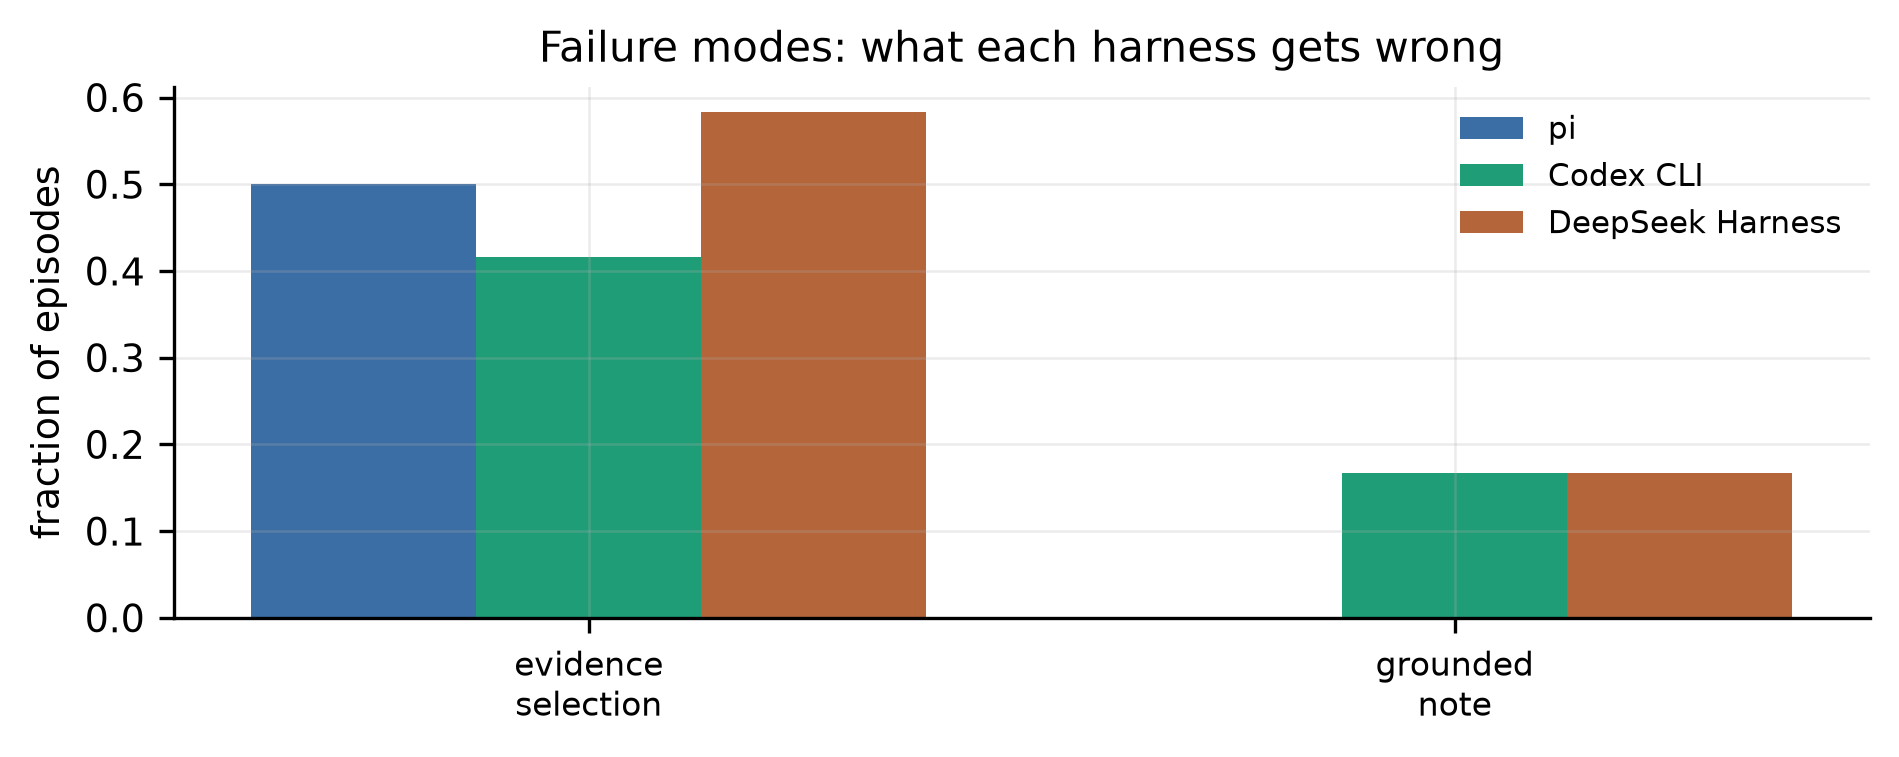
\includegraphics[keepaspectratio,alt={Which verifier checks each harness actually misses, as a fraction of its episodes.}]{figures/fig4-failure-modes.png}}
\caption{Which verifier checks each harness actually misses, as a
fraction of its episodes.}
\end{figure}

\subsubsection{5.6 What the comparison does and does not
show}\label{what-the-comparison-does-and-does-not-show}

It shows that tasks compiled by HealthEnv are solvable by three
independently built agent loops that were never adapted to this
benchmark, through one narrow tool surface, with scoring done offline.
It shows that the measured differences are attributable to the loop,
because the model, the sample, the prompt, and the tools were held
identical.

It does not show that the harnesses differ \emph{in general} --- the
sample is small, and a single model on a single endpoint cannot separate
loop quality from how well that loop happens to suit one model. It does
not compare model capability, since all three run the same weights. It
does not measure GUI grounding, because the harnesses call an HTTP API
rather than a rendered interface; the browser layer is proved separately
and exhaustively over all 1200 tasks in Section 4.3, but the harness
comparison is not conducted through it. That separation is deliberate
--- it isolates ``can the loop read, select, and act on evidence'' from
``can the agent ground a rendered interface'' --- and it also means the
two results must not be conflated: 1200/1200 in the browser does not
imply the harnesses would score well under a pixel-input interface, and
vice versa.

\subsection{6. Relation to prior work}\label{relation-to-prior-work}

\subsubsection{Health reasoning
benchmarks}\label{health-reasoning-benchmarks}

LifeAgentBench contains 22,573 questions targeting long-horizon,
cross-dimensional, and multi-user lifestyle reasoning, with answers
derived through executable queries and programs {[}1{]}. HealthEnv uses
the resulting QA relation as a seed for interaction rather than as the
final evaluation surface.

\subsubsection{Medical computer-use
benchmarks}\label{medical-computer-use-benchmarks}

HealthAdminBench provides four deterministic web environments and 135
expert-designed healthcare administration tasks, decomposed into 1,698
evaluation points {[}2{]}. MedCUA-Bench covers 18 clinical scenarios
across 10 medical domains and evaluates task completion plus five
clinical safety dimensions {[}3{]}. These works define the target
standard for realistic workflows and safety-aware scoring. HealthEnv
differs in source and purpose: it starts from existing QA relations and
studies automatic expansion.

\subsubsection{Environment synthesis}\label{environment-synthesis}

InfiniteWeb combines unified specification and task-centric test-driven
development to generate functional websites and evaluators {[}4{]}.
AutoWebWorld represents websites as finite-state machines, making
transitions and goal states programmatically verifiable {[}5{]}.
GUI-GENESIS reconstructs efficient GUI environments with verifiable
rewards {[}6{]}. CUA-Gym co-generates instructions, environment states,
and reward functions, while separating generator and discriminator roles
{[}7{]}. Gym-Anything treats software-environment creation as a
multi-agent build-and-audit problem {[}8{]}. FaraGen1.5 organizes
generation around environments, solvers, and complementary verifiers
{[}9{]}.

HealthEnv adopts their shared principle---environment generation must be
coupled to verification---but introduces a domain-specific seed:
executable health QA.

\subsubsection{Agent harnesses as a measurement
variable}\label{agent-harnesses-as-a-measurement-variable}

Agent harnesses---the loop around a model, comprising the scaffold, tool
vocabulary, context policy, shell, and stop condition---have become
first-class artifacts in their own right. Terminal-Bench and similar
agentic benchmarks have made the harness an explicit component of the
evaluated system, and harnesses such as \texttt{pi}, Codex CLI, and
\texttt{dsh} are distributed and versioned independently of any model.
This creates a measurement problem that text benchmarks do not have: a
score is a property of the pair (model, harness), and a benchmark that
does not control the harness cannot attribute a difference to either.
HealthEnv's contribution here is narrow and empirical --- one model, one
sample, one prompt, one tool surface, three harnesses --- and its value
is as much in the documented hazards (Section 5.3) as in the numbers,
since those hazards corrupt the comparison without changing its apparent
plausibility.

\subsection{7. Research agenda}\label{research-agenda}

A full paper should test four hypotheses.

\textbf{H1: Expansion fidelity.} Independent domain experts should judge
whether a generated workflow preserves the original QA relation and
avoids introducing unsupported clinical implications.

\textbf{H2: Verifier validity.} Counterexample policies should fail.
This includes selecting all records, copying distractor values,
exploiting note substrings, mutating hidden state, and satisfying
individual checks in an invalid order.

\textbf{H3: Environment diversity.} Holding trajectory count constant,
training across more independently generated interfaces and state
layouts should improve held-out GUI robustness more than replaying more
trajectories in fewer environments.

\textbf{H4: Transfer.} Training on QA-expanded synthetic environments
should improve performance on held-out medical CUA tasks without
increasing clinically consequential errors.

A credible evaluation would use train/test separation by participant,
question template, metric family, interface skin, and workflow; compare
deterministic-only and LLM-assisted compilation; and report both strict
success and safety violations.

\subsection{8. Safety, ethics, and
governance}\label{safety-ethics-and-governance}

HealthEnv can create high-stakes-looking interfaces. That makes scope
control essential.

\begin{itemize}
\tightlist
\item
  The public artifact contains synthetic data only.
\item
  The action space excludes diagnosis, treatment, prescription, and
  communication with real patients.
\item
  Demonstrations should be labeled as simulations.
\item
  Dataset licenses and data-use agreements must be checked before
  conversion.
\item
  PHI must not be sent to external model APIs.
\item
  Realistic environments need red-team evaluation for reward hacking,
  unsafe documentation, and automation bias.
\item
  Human review remains necessary before any deployment-adjacent use.
\end{itemize}

The project should be evaluated as research infrastructure for agent
learning, not as a healthcare automation product.

\subsection{9. Limitations}\label{limitations}

The prototype has three browser surface skins over one application, a
narrow record schema, handcrafted action primitives, and term-based note
checking. It does not model authentication, role permissions,
cross-application document transfer, asynchronous workflows, or clinical
ontologies. Its LifeAgentBench adapter currently handles dated numeric
comparison items and synthesizes evidence states rather than
reconstructing the original database.

The cross-harness comparison has its own bounds. It runs a single model
on a single endpoint, so it separates loops only relative to that model;
it cannot rank the harnesses in general. The harnesses drive the
environment through an HTTP tool API rather than a rendered interface,
so this section measures the loop's ability to read, select, and act on
evidence --- not its pixel-level GUI grounding, which the browser layer
exercises separately. The sample is 12 tasks per harness, which is
enough to distinguish ``works'' from ``cannot start'' but not enough for
confidence intervals on small differences. One harness needed a sandbox
mode widened and another needed its shell path supplied; those are
configuration changes to make the agents runnable at all, and they are
disclosed rather than smoothed over.

These limitations are not cosmetic. They define the next implementation
milestones and the difference between a working compiler prototype and a
publishable empirical result.

\subsection{10. Conclusion}\label{conclusion}

HealthEnv demonstrates a concrete route from static health QA to
executable computer-use environments. The central mechanism is not the
UI generator alone; it is the separation of seed truth, planner
language, runtime state, and verifier logic. The released vertical slice
establishes that this separation can be implemented, tested, and audited
with minimal infrastructure, and that the resulting tasks are robust
enough to compare three independently built agent harnesses under
controlled conditions. The next question is empirical: whether scaling
this compilation process yields environments that are diverse enough to
train agents and faithful enough to trust.

\subsection{References}\label{references}

\begin{enumerate}
\def\labelenumi{\arabic{enumi}.}
\tightlist
\item
  Ye Tian, Zihao Wang, Onat Gungor, Xiaoran Fan, and Tajana Rosing.
  ``LifeAgentBench: Benchmarking LLMs for Long-Horizon,
  Cross-Dimensional Lifestyle Health Reasoning.'' arXiv:2601.13880,
  2026. \url{https://arxiv.org/abs/2601.13880}
\item
  Suhana Bedi et al.~``HealthAdminBench: Evaluating Computer-Use Agents
  on Healthcare Administration Tasks.'' arXiv:2604.09937, 2026.
  \url{https://arxiv.org/abs/2604.09937}
\item
  Jia Yu, Zilong Wang, Xinyang Jiang, Dongsheng Li, and Shuo Wang.
  ``MedCUA-Bench: A Screenshot-Only Benchmark for Clinical Computer-Use
  Agents.'' arXiv:2606.03203, 2026.
  \url{https://arxiv.org/abs/2606.03203}
\item
  Ziyun Zhang et al.~``InfiniteWeb: Scalable Web Environment Synthesis
  for GUI Agent Training.'' arXiv:2601.04126, 2026.
  \url{https://arxiv.org/abs/2601.04126}
\item
  Yifan Wu et al.~``AutoWebWorld: Synthesizing Infinite Verifiable Web
  Environments via Finite State Machines.'' arXiv:2602.14296, 2026.
  \url{https://arxiv.org/abs/2602.14296}
\item
  Yuan Cao et al.~``GUI-GENESIS: Automated Synthesis of Efficient
  Environments with Verifiable Rewards for GUI Agent Post-Training.''
  arXiv:2602.14093, 2026. \url{https://arxiv.org/abs/2602.14093}
\item
  Bowen Wang et al.~``CUA-Gym: Scaling Verifiable Training Environments
  and Tasks for Computer-Use Agents.'' arXiv:2605.25624, 2026.
  \url{https://arxiv.org/abs/2605.25624}
\item
  Pranjal Aggarwal, Graham Neubig, and Sean Welleck. ``Gym-Anything:
  Turn any Software into an Agent Environment.'' arXiv:2604.06126, 2026.
  \url{https://arxiv.org/abs/2604.06126}
\item
  Ahmed Awadallah et al.~``Fara-1.5: Scalable Learning Environments for
  Computer Use Agents.'' arXiv:2606.20785, 2026.
  \url{https://arxiv.org/abs/2606.20785}
\end{enumerate}

\bibliography{references.bib}

\end{document}
